\documentclass[11pt,a4paper]{article}

\usepackage{amsmath}
\usepackage{amssymb}
\usepackage{graphicx}
\usepackage{geometry}
\usepackage{hyperref}
\usepackage{listings}
\usepackage{xcolor}
\usepackage[utf8]{inputenc}
\usepackage[T1]{fontenc}
\usepackage{booktabs}
\usepackage{array}
\usepackage{tabularx}
\usepackage{enumitem}
\usepackage{tikz}
\usepackage{pgfplots}
\pgfplotsset{compat=1.18}
\usepackage{multirow}
\usepackage{colortbl}
\usepackage{parskip}
\usepackage{mdframed}
\usepackage{tcolorbox}
\tcbuselibrary{skins}

\geometry{margin=2.5cm}
\renewcommand{\arraystretch}{1}
\title{Commodity Forward Curve Analytics Platform}
\author{Adam El Gbouri}
\date{April 2026}
\renewcommand{\arraystretch}{1}

\definecolor{amber}{RGB}{240,165,0}
\definecolor{accentblue}{RGB}{31,111,235}
\definecolor{lightgray}{RGB}{246,248,250}
\definecolor{darktext}{RGB}{26,26,46}
\definecolor{signalgreen}{RGB}{26,127,55}
\definecolor{signalred}{RGB}{207,34,46}
\definecolor{signalgray}{RGB}{110,118,129}
\definecolor{boxbg}{RGB}{237,244,255}
\definecolor{notebg}{RGB}{255,251,235}
\definecolor{noteborder}{RGB}{240,165,0}

\renewcommand{\arraystretch}{1.45}

\lstset{
language=Python,
basicstyle=\ttfamily\small,
keywordstyle=\color{accentblue},
commentstyle=\color{signalgray},
stringstyle=\color{amber},
breaklines=true,
backgroundcolor=\color{lightgray},
frame=single,
framerule=0.4pt,
rulecolor=\color{signalgray},
xleftmargin=8pt,
xrightmargin=8pt
}

\newenvironment{keybox}[1]{%
  \begin{tcolorbox}[
    colback=boxbg, colframe=accentblue,
    fonttitle=\bfseries\small, title=#1,
    left=8pt, right=8pt, top=6pt, bottom=6pt, boxrule=0.5pt
  ]
}{\end{tcolorbox}}

\newenvironment{notebox}{%
  \begin{tcolorbox}[
    colback=notebg, colframe=noteborder,
    left=8pt, right=8pt, top=5pt, bottom=5pt, boxrule=0.5pt
  ]
}{\end{tcolorbox}}


\begin{document}

\maketitle

% =============================================================================
\section{Introduction}
% =============================================================================

\subsection{What is a Forward Curve?}

When a commodity is traded on a futures exchange, it is not only the current price that is visible --- dozens of contracts with different delivery dates are quoted simultaneously. The set of all these prices, plotted against their maturity, forms what is called a \textbf{forward curve}.

The shape of this curve is not random. It directly reflects the market's collective view of supply, demand, and storage conditions over the coming months. Two fundamental structures exist:

\medskip
\begin{center}
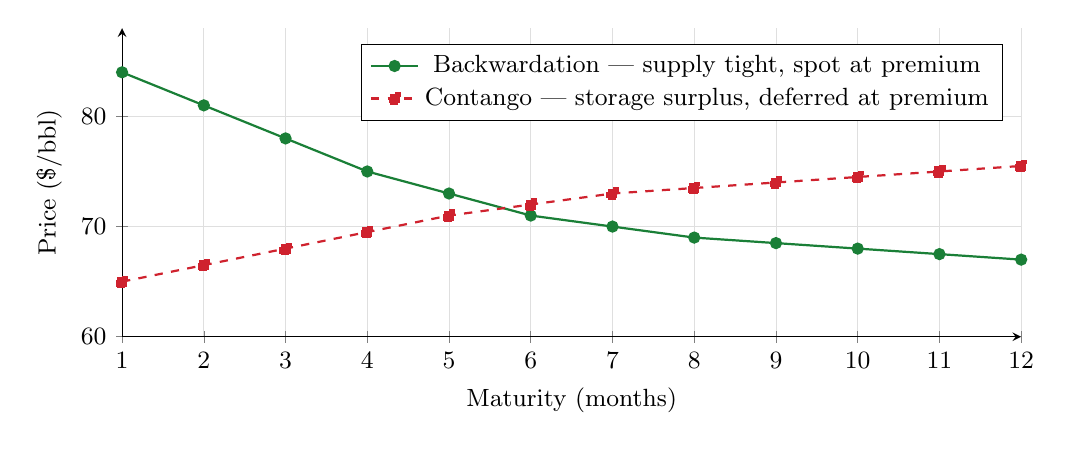
\begin{tikzpicture}
\begin{axis}[
    width=13cm, height=5.5cm,
    xlabel={Maturity (months)},
    ylabel={Price (\$/bbl)},
    xmin=1, xmax=12, ymin=60, ymax=88,
    xtick={1,2,3,4,5,6,7,8,9,10,11,12},
    grid=both, grid style={line width=0.3pt, draw=gray!25},
    axis lines=left,
    tick label style={font=\small}, label style={font=\small},
    legend style={font=\small, at={(0.98,0.95)}, anchor=north east}
]
\addplot[color=signalgreen, thick, mark=*, mark size=1.8pt]
    coordinates {(1,84)(2,81)(3,78)(4,75)(5,73)(6,71)(7,70)(8,69)(9,68.5)(10,68)(11,67.5)(12,67)};
\addlegendentry{Backwardation --- supply tight, spot at premium}
\addplot[color=signalred, thick, mark=square*, mark size=1.8pt, dashed]
    coordinates {(1,65)(2,66.5)(3,68)(4,69.5)(5,71)(6,72)(7,73)(8,73.5)(9,74)(10,74.5)(11,75)(12,75.5)};
\addlegendentry{Contango --- storage surplus, deferred at premium}
\end{axis}
\end{tikzpicture}
\end{center}
\begin{center}{\small\textit{Figure 1: The two main forward curve structures.}}\end{center}

\begin{keybox}{Key definitions}
\textbf{Backwardation}: near-term prices higher than deferred prices. The market is paying a premium for immediate delivery, signalling tight supply or low inventories.\\[4pt]
\textbf{Contango}: deferred prices higher than near-term prices. Storage costs and a comfortable supply balance push future prices above today's spot.
\end{keybox}

\subsection{Why Does It Matter?}

Reading the forward curve correctly allows traders, risk managers and industrial buyers to answer practical questions every day:

\begin{itemize}[itemsep=4pt]
\item Is the market tight right now, or are inventories building?
\item Should I lock in a fixed price today, or wait for deferred contracts?
\item Does the market expect the current price level to persist, or to mean-revert?
\item What is the implied cost of rolling a long futures position forward each month?
\end{itemize}

\subsection{What is CFCAP?}

\textbf{CFCAP} (Commodity Forward Curve Analytics Platform) is a Python application that automates the full analysis pipeline: it downloads live futures prices, fits quantitative models to the forward curve, computes financial metrics, generates trading signals, and presents all results in an interactive Streamlit dashboard.

It covers more than \textbf{65 commodities} across 8 asset classes, from WTI Crude Oil to LME Nickel, EU Carbon allowances and Baltic freight rates.

% =============================================================================
\section{Architecture and Usage}
% =============================================================================

\subsection{Streamlit-Only Design}

In this updated version, CFCAP runs exclusively as a \textbf{Streamlit web application}. The entire platform is contained in a single Python file, \texttt{cfcap.py}.

\begin{center}
\begin{tabularx}{\textwidth}{>{\bfseries}l X l}
\toprule
Mode & Description & How to launch \\
\midrule
Streamlit dashboard & Full browser interface with interactive Plotly charts & \texttt{streamlit run cfcap.py} \\
CLI single run      & One commodity, automated, no interaction needed & \texttt{python cfcap.py -{}-commodity X} \\
Daily scheduler     & Batch of 11 commodities every morning at 09:15 EST & \texttt{python cfcap.py -{}-schedule} \\
\bottomrule
\end{tabularx}
\end{center}

\subsection{The Analysis Pipeline}

Every run follows the same six-step pipeline:

\medskip
\begin{center}
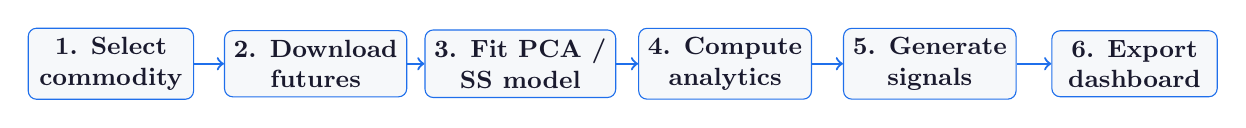
\begin{tikzpicture}[
    box/.style={draw=accentblue, fill=lightgray, rounded corners=3pt,
                minimum width=2.1cm, minimum height=0.8cm,
                font=\small\bfseries, text=darktext, align=center},
    arrow/.style={->, thick, color=accentblue}
]
\node[box] (A) at (0,0)    {1. Select\\commodity};
\node[box] (B) at (2.6,0)  {2. Download\\futures};
\node[box] (C) at (5.2,0)  {3. Fit PCA /\\SS model};
\node[box] (D) at (7.8,0)  {4. Compute\\analytics};
\node[box] (E) at (10.4,0) {5. Generate\\signals};
\node[box] (F) at (13.0,0) {6. Export\\dashboard};
\draw[arrow] (A) -- (B);
\draw[arrow] (B) -- (C);
\draw[arrow] (C) -- (D);
\draw[arrow] (D) -- (E);
\draw[arrow] (E) -- (F);
\end{tikzpicture}
\end{center}

\subsection{Technologies and Libraries}

\begin{center}
\begin{tabularx}{\textwidth}{>{\ttfamily\bfseries}l >{\bfseries}l X}
\toprule
\normalfont\textbf{Library} & Role & Purpose in CFCAP \\
\midrule
numpy        & Numerics      & Curve fitting, yield computations, VaR estimates \\
pandas       & Data          & Forward curve DataFrames, CSV snapshots, historical loads \\
scipy        & Optimisation  & \texttt{least\_squares} for Schwartz-Smith, cubic spline interpolation \\
scikit-learn & Machine learn.& PCA decomposition of the forward curve \\
matplotlib   & Visualisation & Static 4-panel PNG dashboard \\
yfinance     & Market data   & Live futures prices (NYMEX, COMEX, CBOT, ICE) \\
tvdatafeed   & Market data   & TradingView contracts: LME, TTF, Jet Kero, Carbon \\
streamlit    & Dashboard     & Interactive browser interface \\
plotly       & Charts        & Zoomable, hoverable charts in Streamlit \\
requests     & API           & EIA Open Data: crude and gas inventories, production \\
schedule     & Automation    & Daily batch scheduler \\
\bottomrule
\end{tabularx}
\end{center}

% =============================================================================
\section{Commodities Covered}
% =============================================================================

The commodity registry covers 65 instruments. Each entry stores its data source, CME month codes, ticker format, storage cost, and model fitting bounds. The program routes each download automatically.

\begin{center}
\begin{tabularx}{\textwidth}{>{\bfseries}l c c X}
\toprule
Family & Count & Source & Examples \\
\midrule
Energy              & 9  & Yahoo Finance  & WTI, Brent, Natural Gas, RBOB, Heating Oil, Gasoil, Jet Kero \\
Metals              & 5  & Yahoo Finance  & Gold, Silver, Copper, Platinum, Palladium \\
Agriculture         & 15 & Yahoo Finance  & Corn, Wheat, Soybeans, Sugar, Coffee, Cocoa, Cattle, Hogs \\
Base Metals (LME)   & 10 & TradingView    & Copper, Aluminum, Zinc, Nickel, Lead, Tin, Cobalt, Lithium \\
Energy (additional) & 10 & TradingView    & TTF, NBP, Coal API2/4, Uranium, Carbon EUA, Naphtha \\
Freight             & 4  & TradingView    & Capesize, Panamax, Supramax, VLCC Tanker \\
Carbon              & 4  & TradingView    & EU EUA, UK UKA, California CCA, RGGI \\
Dairy \& Tropical   & 8  & Yahoo / TV     & Palm Oil, Canola, Milk, Butter, Robusta Coffee \\
\midrule
\textbf{Total}      & \textbf{65+} & & \\
\bottomrule
\end{tabularx}
\end{center}

\begin{notebox}
\textbf{Data routing:} Yahoo Finance is used for most exchange-traded contracts via a single grouped download. TradingView is used for ICE London, LME and other contracts not available on Yahoo. The routing is automatic and transparent.
\end{notebox}

% =============================================================================
\section{Forward Curve Analytics}
% =============================================================================

\subsection{Convenience Yield}

The convenience yield is one of the most important quantities in commodity finance. It measures the implied benefit of holding the \textit{physical} commodity rather than a futures contract.

It is derived by inverting the cost-of-carry equation:

\begin{equation}
F(T) = S \cdot e^{(r + u - cy)\,T}
\quad \Longrightarrow \quad
cy(T) = r + u - \frac{1}{T}\ln\!\left(\frac{F(T)}{S}\right)
\end{equation}

where $r$ is the risk-free rate, $u$ the annualised storage cost, and $S$ the spot price.

\begin{center}
\begin{tabularx}{\textwidth}{l l X}
\toprule
Condition & Signal & Economic interpretation \\
\midrule
$cy > 2 \times r$ & \textcolor{signalgreen}{\textbf{BUY}} & The market pays a large premium for physical ownership. Inventories are low, supply is tight. \\
$r < cy < 2 \times r$ & Neutral & Positive carry, but not strong enough to drive aggressive accumulation. \\
$0 < cy < r$ & Neutral & Positive but below financing cost. Physical storage barely economic. \\
$cy < 0$ & \textcolor{signalred}{\textbf{SELL}} & Forward premium exceeds all carry costs. Classic cash-and-carry arbitrage opportunity. \\
\bottomrule
\end{tabularx}
\end{center}

\subsection{Roll Yield}

\begin{equation}
ry(T) = \frac{S - F(T)}{F(T) \cdot T}
\end{equation}

In backwardation, the roll yield is positive and rewards passive long investors.
In contango, it is negative and erodes returns by 10--15\% per year for commodity ETFs.

\subsection{Calendar Spreads}

\[
\text{Spread}_{i \to j} = F(T_j) - F(T_i), \quad T_j > T_i
\]

CFCAP computes all consecutive M+1 spreads along the curve and counts how many months are in each regime, highlighting the most significant legs for calendar spread trades.

% =============================================================================
\section{Quantitative Models}
% =============================================================================

In this section we will discuss the implementation of two powerful approaches: Principal Component Analysis (PCA) and the Schwartz-Smith 3-factor model. Both are accessible via dedicated tabs in the Streamlit dashboard.

% -----------------------------------------------------------------------------
\subsection{Principal Component Analysis (PCA)}
% -----------------------------------------------------------------------------

\subsubsection{Motivation}

PCA is a data-driven approach that identifies the \textit{directions of maximum variance} in the forward curve. Rather than imposing a parametric shape (as other models do), PCA discovers the empirical structure of curve movements from historical data.

Applied to commodity forward curves, PCA consistently identifies three dominant factors that together explain more than 95\% of all price variance across maturities.

\subsubsection{Methodology}

A matrix of 50 synthetic historical observations is constructed around today's curve using three types of perturbation:

\begin{equation}
\tilde{F}^{(k)}(T) = F(T) + \underbrace{\delta_{\text{level}}}_{\text{parallel shift}}
                             + \underbrace{\delta_{\text{slope}} \cdot T}_{\text{twist}}
                             + \underbrace{\delta_{\text{hump}} \cdot e^{-(T-\bar{T})^2/2\sigma_T^2}}_{\text{curvature}}
                             + \underbrace{\varepsilon(T)}_{\text{idiosyncratic}}
\end{equation}

The idiosyncratic noise $\varepsilon(T) \sim \mathcal{N}(0,\, 0.002 \cdot S)$ per contract ensures the covariance matrix is full-rank, producing a meaningful out-of-sample RMSE.

PCA is then fitted on the training set (without today's curve), and today's curve is
projected onto the principal component space:

\begin{equation}
\hat{F}(T) = \bar{F}(T) + \sum_{k=1}^{K} z_k \cdot \mathbf{v}_k(T)
\end{equation}

where $z_k = \langle F - \bar{F},\, \mathbf{v}_k \rangle$ are the scores and
$\mathbf{v}_k$ the eigenvectors.

\subsubsection{The Three Principal Components}

\begin{center}
\begin{tabularx}{\textwidth}{c >{\bfseries}l X l}
\toprule
PC & Name & Economic meaning & Typical variance \\
\midrule
PC1 & Level     & Uniform shift of all maturities simultaneously. Driven by macro events, dollar moves, or OPEC decisions that affect the entire curve in parallel. & $\sim$75\% \\
PC2 & Slope     & Steepening or flattening: front end moves more than back end, or vice versa. Reflects supply shocks concentrated at prompt maturities or structural regime changes. & $\sim$15\% \\
PC3 & Curvature & Belly vs.\ wings: the middle of the curve moves relative to both ends. Typical of seasonal patterns or short-term delivery constraints at specific maturities. & $\sim$7\% \\
\bottomrule
\end{tabularx}
\end{center}

\begin{notebox}
\textbf{Interpretation example:} A positive PC2 score means the front end of the WTI curve is relatively elevated compared to the back end --- a steepening / backwardation signal. A negative PC2 score indicates the back end has risen more --- a flattening or contango pressure signal. The score is updated every time new data is loaded.
\end{notebox}

\subsubsection{Dashboard Output}

The PCA tab displays two charts:
\begin{itemize}[itemsep=3pt]
\item \textbf{Reconstruction chart}: observed prices vs.\ PCA reconstruction, with RMSE
\item \textbf{Loadings chart}: the shape of each principal component across all maturities
\end{itemize}
The right panel shows the score (projection value), explained variance, and cumulative
variance for each component.

% -----------------------------------------------------------------------------
\subsection{Schwartz-Smith 3-Factor Model}
% -----------------------------------------------------------------------------

\subsubsection{Motivation}

The Schwartz-Smith model (2000) is a continuous-time stochastic model that decomposes the log-price of a futures contract into three economically interpretable factors. Unlike PCA, it provides a \textit{structural} decomposition with clear meaning for each component, making it directly usable for pricing, hedging, and risk management.

\subsubsection{Model Specification}

The log futures price at maturity $T$ is decomposed as:

\begin{equation}
\ln F(T) = \underbrace{\chi(T)}_{\text{short-term deviation}}
         + \underbrace{\xi_0}_{\text{long-term equilibrium}}
         + \underbrace{A \cdot \sin(\omega T + \phi_0)}_{\text{seasonal component}}
\end{equation}

where:

\begin{itemize}[itemsep=4pt]
\item $\chi(T) = \chi_0 \cdot e^{-\kappa T}$ is the short-term deviation from equilibrium,
      mean-reverting at speed $\kappa$ (per year). It captures prompt supply shocks,
      weather events, or temporary demand spikes that fade over time.

\item $\xi_0$ is the long-term equilibrium log-price. Its exponential $e^{\xi_0}$ gives
      the long-run fair value of the commodity --- where the market expects prices to
      converge as all transient shocks dissipate.

\item $A \cdot \sin(\omega T + \phi_0)$ is a seasonal component with amplitude $A$,
      frequency $\omega$ (radians per year), and phase $\phi_0$. It captures systematic
      seasonal patterns such as winter gas demand or summer gasoline demand.
\end{itemize}

\subsubsection{Parameters and Economic Interpretation}

\begin{center}
\begin{tabularx}{\textwidth}{c >{\bfseries}l X l}
\toprule
Param. & Name & Economic meaning & Typical value (WTI) \\
\midrule
$\xi_0$ & Long-term equilibrium & Log-price of the long-run fair value. $e^{\xi_0}$ gives the equilibrium price in \$/bbl. The market converges toward this level as all shocks fade. & $\ln(65) \approx 4.17$ \\
$\chi_0$ & Spot deviation & How far today's spot deviates from $\xi_0$. Positive means spot is above equilibrium (tight market); negative means below (surplus). & $+0.08$ \\
$\kappa$ & Mean-reversion speed & How quickly $\chi(T)$ reverts to zero. High $\kappa$ = shock dissipates in months; low $\kappa$ = persistent deviation. Half-life $= \ln 2/\kappa$. & $2.5$ /yr \\
Half-life & --- & Time for $\chi$ to lose half its value: $\ln(2)/\kappa$. Directly interpretable: a half-life of 3 months means prompt shocks fade within a quarter. & $0.28$ yr (3.3 mo) \\
$A$ & Seasonal amplitude & Magnitude of the seasonal cycle as a fraction of $\ln F$. Larger for natural gas than crude oil. & $0.03$ \\
$\omega$ & Seasonal frequency & $2\pi$ = one full cycle per year. Values near $4\pi$ indicate two cycles (e.g.\ winter + summer peaks). & $2\pi$ rad/yr \\
\bottomrule
\end{tabularx}
\end{center}

\subsubsection{Calibration}

The model is calibrated by nonlinear least squares on the observed cross-section
of futures prices using \texttt{scipy.optimize.least\_squares}:

\begin{equation}
\min_{\chi_0,\, \kappa,\, \xi_0,\, A,\, \omega,\, \phi_0}
\sum_{i=1}^{N} \bigl[\ln F(T_i) - \chi_0 e^{-\kappa T_i} - \xi_0
                     - A\sin(\omega T_i + \phi_0)\bigr]^2
\end{equation}

The RMSE is computed in price space (not log-price) against the observed futures prices,
providing a directly comparable measure of fit quality.

\subsubsection{Dashboard Output}

The Schwartz-Smith tab displays:
\begin{itemize}[itemsep=3pt]
\item \textbf{Fit chart}: observed prices vs.\ SS fitted curve, with the $e^{\xi_0}$
      equilibrium line
\item \textbf{Factor decomposition}: bar chart of $\chi(T)$ and seasonal contributions
      by maturity
\item \textbf{Parameter panel}: all 7 parameters with their economic interpretation
\end{itemize}

\subsubsection{Comparison: PCA vs.\ Schwartz-Smith}

\begin{center}
\begin{tabularx}{\textwidth}{l X X}
\toprule
& \textbf{PCA} & \textbf{Schwartz-Smith} \\
\midrule
Approach      & Data-driven (statistical) & Structural (financial theory) \\
Parameters    & Component scores (dimensionless) & Physical parameters ($\kappa$, $\xi_0$, half-life) \\
Best for      & Detecting dominant curve movements, relative value & Pricing derivatives, hedging, equilibrium estimation \\
Extrapolation & Cannot extrapolate beyond observed maturities & Can extrapolate: $\chi \to 0$ as $T \to \infty$ \\
Interpretation & ``PC2 score = $+0.45$'' (relative) & ``Half-life = 3.3 months'' (absolute, intuitive) \\
RMSE          & Out-of-sample (honest reconstruction error) & In-sample fit of the log-price cross-section \\
\bottomrule
\end{tabularx}
\end{center}

% =============================================================================
\section{Trading Signal Engine}
% =============================================================================

\subsection{Overview}

The signal engine evaluates \textbf{51 rule-based conditions} against the live analytics and produces actionable outputs with a plain-language rationale.

Every signal card shows:
\begin{itemize}[itemsep=2pt]
\item The \textbf{signal level}: BUY, SELL, SPREAD, HEDGE, ARBITRAGE, WARNING, or NEUTRAL
\item The \textbf{trigger values}: the exact numbers that activated the rule
\item The \textbf{rationale}: a short explanation of why the condition is significant
\end{itemize}

\subsection{Signal Categories}

\begin{center}
\begin{tabularx}{\textwidth}{>{\bfseries}l c X}
\toprule
Category & Signals & What it detects \\
\midrule
Convenience Yield   & 6 & $cy > 2.5r$: physical accumulation. $cy < 0$: cash-and-carry arbitrage. CY term structure steepening or flattening. \\
Roll Yield          & 6 & $ry > 8\%$/yr: rewards long exposure. $ry < -8\%$/yr: passive long drag. Net carry cost vs.\ convenience yield. \\
Calendar Spreads    & 8 & M1-M2, M1-M3, M1-M6 spreads against spot thresholds. Mixed structure. Butterfly spreads. \\
Schwartz-Smith      & 6 & Spot vs.\ $e^{\xi_0}$ equilibrium (mean reversion). Half-life of short-term deviation. Seasonal amplitude signal. \\
Structural Regime   & 5 & Proportion of curve in backwardation or contango, from mild ($\geq 60\%$) to deep ($\geq 85\%$). \\
Temporal (J-7/J-14) & 6 & Price momentum over 7 days. Curve twist (front vs.\ back shift). Parallel shift detection. \\
Hedger Signals      & 3 & Producer sell-forward opportunity. Consumer fixed-price buying. Collar strategy. \\
Arbitrage           & 2 & Actual forward vs.\ theoretical $S \cdot e^{(r+u)T}$. Reverse cash-and-carry. \\
Curve Shape         & 3 & $R^2 < 0.75$: kink detected. High model residuals. Implied volatility from steepness. \\
Risk                & 2 & $\sigma_{\text{ann}} = \frac{|\Delta S_{7d}|}{7}\sqrt{252}$. VaR at 95\% and 99\% from 7-day move. \\
Summary             & 2 & $\geq 3$ aligned signals $\Rightarrow$ \textcolor{signalgreen}{\textbf{STRONG BUY}} or \textcolor{signalred}{\textbf{STRONG SELL}}. \\
\midrule
\textbf{Total} & \textbf{51} & \\
\bottomrule
\end{tabularx}
\end{center}

\begin{notebox}
\textbf{Model integration in signals:} The Schwartz-Smith equilibrium $e^{\xi_0}$ represents the long-run fair value anchor. When spot is more than 12\% above $e^{\xi_0}$, a mean-reversion SELL signal fires. When spot is more than 12\% below, a mean-reversion BUY signal fires. The half-life of $\chi$ controls whether the signal is flagged as a short-term opportunity (half-life $<$ 4 months) or a structural dislocation (half-life $>$ 12 months).
\end{notebox}

% =============================================================================
\section{EIA Fundamental Data}
% =============================================================================

For energy commodities, CFCAP integrates fundamental context through the
\textbf{EIA Open Data API}.

\begin{center}
\begin{tabularx}{\textwidth}{>{\bfseries}l l X}
\toprule
Series & Unit & Why it matters \\
\midrule
Cushing crude stocks    & kbbl   & Key WTI delivery point. Falling stocks support backwardation; rising stocks drive contango. \\
US total crude stocks   & kbbl   & Broad supply picture. A 3-week consecutive build is a bearish signal. \\
US crude production     & kbbl/d & Higher production supports contango through supply pressure. \\
WTI / Brent spot        & \$/bbl & Cross-check against downloaded futures to detect data errors. \\
US refinery utilisation & \%     & Low utilisation means crude accumulates; high utilisation supports backwardation. \\
US natural gas storage  & Bcf    & Below 5-year average: bullish for TTF and Henry Hub. \\
\bottomrule
\end{tabularx}
\end{center}

\begin{notebox}
\textbf{Practical example:} If Cushing stocks have fallen for four consecutive weeks and the WTI curve is in strong backwardation, the EIA panel and the signal engine will both point in the same direction. If they diverge (backwardation but rising stocks), it signals conflicting evidence to investigate further.
\end{notebox}

% =============================================================================
\section{Historical Comparison and Persistence}
% =============================================================================

CFCAP saves a CSV snapshot of every curve it downloads, organised by commodity and date.

\begin{lstlisting}[language=bash]
data/
|-- curves/wti_crude_oil/
|   |-- 2026-04-07.csv    # today
|   |-- 2026-03-31.csv    # 7 days ago
|   |-- 2026-03-24.csv    # 14 days ago
|-- dashboards/wti_crude_oil/
|   |-- wti_crude_oil_20260407_091522.png
|-- eia_cache/            # 24h TTL
|-- logs/scheduler.log
\end{lstlisting}

The Streamlit dashboard includes a \textbf{date selector} in the Forward Curve tab. 
The user can overlay the current curve with any saved snapshot to visualise the exact curve shape before and after any market event.

% =============================================================================
\section{Potential Applications}
% =============================================================================

\begin{center}
\begin{tabularx}{\textwidth}{>{\bfseries}l X}
\toprule
User & How CFCAP helps them \\
\midrule
Energy trader
  & Identify carry trades, detect prompt supply tightening, determine optimal roll maturities, and monitor structural regime changes. The Schwartz-Smith half-life quantifies whether a backwardation episode is transient or structural. \\
Risk manager (airline, refiner, utility)
  & Monitor roll costs, time forward purchases, evaluate collar strategies. The PCA slope score detects steepening/flattening before it is visible in the raw curve. \\
Portfolio manager
  & Assess whether passive long exposure is rewarded by roll yield. Screen commodities by SS equilibrium deviation for mean-reversion trades. \\
Analyst / researcher
  & Compare PCA factor scores across commodities and time. Study how $\kappa$ and half-life vary across commodity cycles. Build historical datasets via the scheduler. \\
Student / practitioner
  & Apply PCA, Schwartz-Smith, cost-of-carry and convenience yield to live market data, with all calculations transparent and documented. \\
\bottomrule
\end{tabularx}
\end{center}

% =============================================================================
\section{Possible Improvements}
% =============================================================================

\subsection{Quantitative Extensions}

\textbf{Full stochastic Schwartz-Smith calibration.}
The current implementation calibrates the SS model on the cross-section of futures prices (static fit). A full Kalman filter calibration would estimate the dynamic state variables $\chi_t$ and $\xi_t$ from time-series data, providing more robust parameter estimates and enabling Monte Carlo simulation for derivative pricing.

\textbf{Asian option pricer.}
Using the SS term structure as the diffusion input, CFCAP could estimate the fair value of Asian calls and puts (options on average price) via Monte Carlo --- directly applicable to jet fuel and crude oil hedging programmes.

\textbf{Historical realised volatility.}
Once sufficient daily snapshots have been saved, rolling 20-day and 60-day realised volatility can be computed. A volatility cone overlaid on the forward curve would help option traders assess whether implied vol is rich or cheap.

\textbf{Portfolio VaR.}
By applying PCA-based curve shocks to a book of futures positions, the platform could compute Value-at-Risk at 95\% and 99\% confidence for a realistic commodity derivatives portfolio.

\subsection{Data and Infrastructure}

\textbf{SQLite database.}
Replacing CSV files with a local SQLite database would enable faster queries, rolling cross-commodity correlation analysis, and multi-date comparisons.

\textbf{FastAPI REST endpoint.}
Exposing analytics as JSON at \texttt{/curve/\{commodity\}} and \texttt{/signals/\{commodity\}} would make the platform consumable by Excel, Power BI, or automated pipelines.

\subsection{User Experience}

\textbf{Morning report.} Automated HTML report sent by email after each scheduler run, containing all charts, signal summaries, and model parameters.

\textbf{Real-time alerts.} Email or Telegram notifications when the SS half-life changes regime (short-term shock vs.\ structural), or when the convenience yield crosses $2 \times r$.

\textbf{Multi-commodity overview.} A landing page showing one row per commodity with spot, structure, roll yield, SS equilibrium deviation, and dominant signal.

% =============================================================================
\section{Conclusion}
% =============================================================================

CFCAP demonstrates how a complete, professional-grade quantitative analytics platform can be built with Python and freely available market data.

The implementation of PCA and Schwartz-Smith represents a significant analytical upgrade. PCA provides a data-driven, model-free decomposition of curve dynamics into interpretable factors. Schwartz-Smith provides a structural, theory-grounded decomposition with directly usable parameters: the long-run equilibrium $e^{\xi_0}$, the mean-reversion speed $\kappa$, and the half-life of transient price shocks.

Together with convenience yield analytics, a 51-signal trading engine, EIA fundamental data, and an interactive Streamlit dashboard, CFCAP provides a rigorous and practical tool for anyone working with commodity derivatives.

\end{document}
